\subsubsection{الگوی \lr{Cyclic Execution}}
\label{archConCyclicExecSec}
\begin{RTL}
الگوی \lr{Cyclic Execution} \cite{ref4} در سیستم‌های کوچک
یا سیستم‌هایی که نیاز به اجرای قابل پیش‌بینی دارند، به طور گسترده‌ای استفاده می‌شود.
این الگو با سادگی و پیش‌بینی‌پذیری خود، پیاده‌سازی آسانی دارد و برای محیط‌های محدود به
حافظه که استفاده از یک سیستم‌عامل بی‌درنگ به طور
کامل عملی نیست، مناسب است. این الگو وظایف
را در یک حلقه ثابت و تکراری اجرا می‌کند و اطمینان می‌دهد که هر
وظیفه به نوبت اجرا می‌شود. سادگی آن نقطه قوت اصلی آن
است، اما انعطاف‌پذیری ندارد و برای رسیدگی به رویدادهای با ضرب‌الاجل‌های
محدود بهینه نیست. وظایف نمی‌توانند در زمان اجرا اضافه یا
حذف شوند و سیستم به تنظیمات زمانی حساس است.
وظایف نادرست می‌توانند کل سیستم را مختل کنند و
الگو در شرایط بار زیاد ناپایدار است. با وجود محدودیت‌ها، برای
سیستم‌های کوچک و پایدار با دینامیک‌های قابل درک مناسب است.
(این الگو همان \nameref{scheduleCyclicExecSec} است که
در \cite{ref1} گفته‌شده.)
\end{RTL}
\begin{figure}[h!]
\centering
\begin{tikzpicture}
    \lr{
        \umlclass[]{Scheluer}{
            \lr{}
        }{
            \lr{}
            }
            \umlclass[x=7]{AbstractThread}{
        }{
            \lr{run()}
            }
            \umlclass[x=5, y=-3]{ConcreteThread}{
            }{
    }    
    \umlassoc[mult1=1, attr2=\{ordered\}|*]{Scheluer}{AbstractThread}
    \umlinherit[]{ConcreteThread}{AbstractThread}
    }
\end{tikzpicture}
\caption{دیاگرام کلاس \lr{Cyclic Execution}}
\label{archConCyclicExecClassDiag}
\end{figure}